%%%%%%%%%%%%%%%%%%%%%%%%%%%%%%%%%%%%%
% Stylish Article
% LaTeX Template
% Version 2.0 (13/4/14)
%
% This template has been downloaded from:
% http://www.LaTeXTemplates.com
%
% Original author:
% Mathias Legrand (legrand.mathias@gmail.com)
%
% License:
% CC BY-NC-SA 3.0 (http://creativecommons.org/licenses/by-nc-sa/3.0/)
%
%%%%%%%%%%%%%%%%%%%%%%%%%%%%%%%%%%%%%%%%%

%----------------------------------------------------------------------------------------
%	PACKAGES AND OTHER DOCUMENT CONFIGURATIONS
%----------------------------------------------------------------------------------------

\documentclass[fleqn,10pt]{SelfArx} % Document font size and equations flushed left
\usepackage[spanish]{babel}

%----------------------------------------------------------------------------------------
%	COLUMNS
%----------------------------------------------------------------------------------------

\setlength{\columnsep}{0.55cm} % Distance between the two columns of text
\setlength{\fboxrule}{0.75pt} % Width of the border around the abstract

%----------------------------------------------------------------------------------------
%	COLORS
%----------------------------------------------------------------------------------------

\definecolor{color1}{RGB}{0,0,90} % Color of the article title and sections
\definecolor{color2}{RGB}{0,20,20} % Color of the boxes behind the abstract and headings

%----------------------------------------------------------------------------------------
%	HYPERLINKS
%----------------------------------------------------------------------------------------

\usepackage{hyperref} % Required for hyperlinks
\usepackage{cite}
\hypersetup{hidelinks,colorlinks,breaklinks=true,urlcolor=color2,citecolor=color1,linkcolor=color1,bookmarksopen=false,pdftitle={Title},pdfauthor={Author}}

%----------------------------------------------------------------------------------------
%	ARTICLE INFORMATION
%----------------------------------------------------------------------------------------

\JournalInfo{Taller de Biotecnología Animal, 2014-I} % Journal information
\Archive{Review} % Additional notes (e.g. copyright, DOI, review/research article)

\PaperTitle{Transfección en Animales} % Article title

\Authors{Juan Manuel Iglesias Artola\textsuperscript{1}, Gianfranco Villamonte Cuneo\textsuperscript{1}} % Authors
\affiliation{\textsuperscript{1}\textit{Facultad de Ciencias Biológicas, Universidad Ricardo Palma, Lima, Peru}} % Author affiliation
%\affiliation{\textsuperscript{2}\textit{Department of Chemistry, University of Examples, London, United Kingdom}} % Author affiliation
\affiliation{*\textbf{Correspondencia}: jmanuel9112@icloud.com / giancuneo@gmail.com } % Corresponding author


%----------------------------------------------------------------------------------------
%	ABSTRACT
%----------------------------------------------------------------------------------------

\Abstract{La transfección es el proceso de introducir nucleótidos en una célula, cuyo producto es la transgénesis. Existen múltiples métodos que permiten realizar esta introducción de nucleótidos, como el uso de vectores virales, nanopartículas mediadoras, o métodos físicos o químicos. Además de aparecer múltiples métodos nuevos de transfección en los últimos años, su eficiencia se sigue incrementando. Esto ha permitido la aparición sin precedentes de un sinnúmero de aplicaciones que plantean nuevas preguntas bioéticas y generan la necesidad de modernizar la reglamentación relacionada.  }


\Keywords{transfección --- transgénicos --- bioética} % Keywords - if you don't want any simply remove all the text between the curly brackets
\newcommand{\keywordname}{Palabras clave} % Defines the keywords heading name

%----------------------------------------------------------------------------------------

\begin{document}

\flushbottom % Makes all text pages the same height

\maketitle % Print the title and abstract box

\tableofcontents % Print the contents section

\thispagestyle{empty} % Removes page numbering from the first page

%----------------------------------------------------------------------------------------
%	ARTICLE CONTENTS
%----------------------------------------------------------------------------------------

\section{Introducción} 

Con la transfección se ha logrado la capacidad de expresar genes de interés en células eucariotas. Esta capacidad ha permitido obtener un mejor entendimiento de la biología celular, la biología molecular y la genética de las células. Al expresar proteínas en células de mamíferos, se ha podido entender aspectos detallados de la síntesis protéica, las interacciones entre proteínas, los efectos de las mutaciones en su función, y las interacciones intercelulares. Además, esta tecnología ha llevado al desarrollo de animales trangénicos, a la fertilización \textit{in vitro}, y a la posibilidad de usar la tranferencia de genes para tratar desórdenes genéticos.

Los virus fueron por mucho tiempo la forma más conveniente de genes a células mamíferas. En 1973 Graham y van der Eb \cite{Graham:1973aa} utilizaron el adenovirus 2 para transfomar células de rata, mientras que en 1984 Cepko et al. \cite{Cepko:1984aa} desarrollaron un retrovirus murínico para la introducción de secuencias de DNA en células mamíferas. Si bien los virus constituyen un medio eficiente para lograr la transfección \textit{in vitro}, la construcción de los vectores es laboriosa, consume tiempo, y tiene diversas limitaciones para su uso \textit{in vivo}.

No obstante la alta eficiencia de la transfección por medio de vectores virales, otros métodos han sido desarrollados. Los trabajos realizados por Pagano et al. fueron pioneros en su área al lograr una alta transferencia de genes a células mamíferas utilizando dietilaminoetil-dextrano (DEAE-D) mezclado con RNA y DNA  \cite{McCutchan:1968aa, Pagano:1967aa}. Después, se demostró que otros métodos también son eficaces: la encapsulación de DNA utilizando liposomas \cite{Fraley:1980aa, Wong:1980aa, Straubinger:1983aa, Fraley:1981aa}, la fusión inducida por polietilenglicol del DNA en los eritrocitos fantasma \cite{Straus:1980aa}, la electroporación \cite{Neumann:1982aa}, los coprecipitados de fosfato de calcio/DNA \cite{Wigler:1979aa}, y los policationes/dimetil sulfóxidos \cite{Kawai:1984aa}. Sin embargo, la eficiencia de los métodos utilizados varía con respecto a las tipos celulares y en general, no fueron muy eficientes y presentaban una alta toxicidad celular.

En la actualidad existen tres grandes grupos de métodos que pueden ser utilizados \cite{Kim:2010aa}: \textit{a)} los métodos biológicos, \textit{b)} los métodos químicos y \textit{c)} los métodos físicos. De estos grupos se pueden emplear métodos que produzcan una transfección pasajero o una integración estable en el genoma del hospedero. En este review se resumen las estrategias experimentales más generales, sus aplicaciones y las implicaciones bioéticas que pueden tener la tranfección de células animales.

%------------------------------------------------

\section{Métodos de Transfección}

\begin{figure*}[ht]\centering % Using \begin{figure*} makes the figure take up the entire width of the page

\includegraphics[width=\linewidth]{images/view}
\caption{Wide Picture}
\label{fig:view}
\end{figure*}


\begin{equation}
\cos^3 \theta =\frac{1}{4}\cos\theta+\frac{3}{4}\cos 3\theta
\label{eq:refname2}
\end{equation}



\begin{enumerate}[noitemsep] % [noitemsep] removes whitespace between the items for a compact look
\item First item in a list
\item Second item in a list
\item Third item in a list
\end{enumerate}

\subsection{Subsection}



\paragraph{Paragraph} %\lipsum[7] % Dummy text
\paragraph{Paragraph} %\lipsum[8] % Dummy text

\subsection{Subsection}

\begin{figure}[ht]\centering
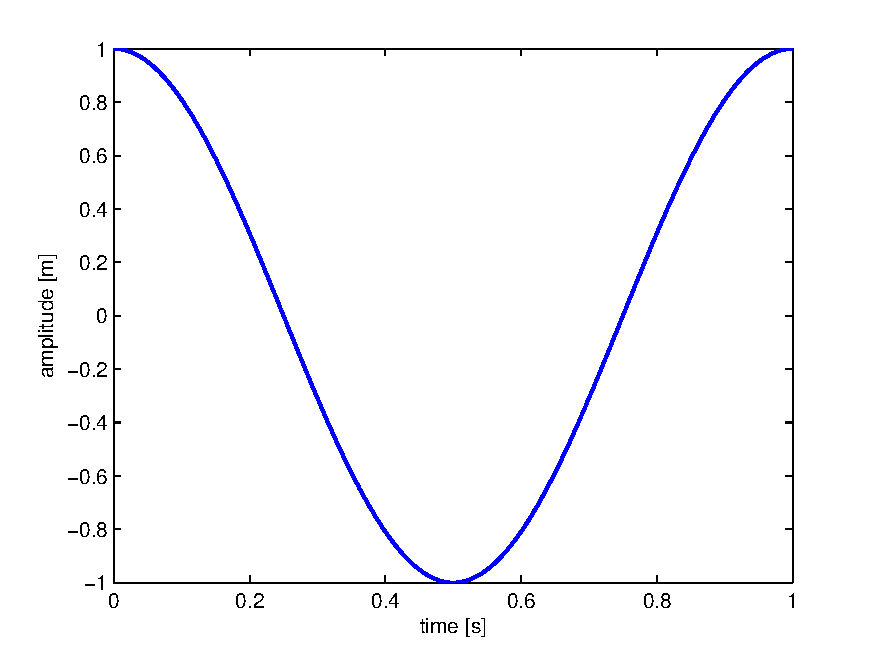
\includegraphics[width=\linewidth]{images/results}
\caption{In-text Picture}
\label{fig:results}
\end{figure}

Reference to Figure \ref{fig:results}.

%------------------------------------------------

\section{Aplicaciones de la Transfección}

La transfección es una herramienta para la modificación genética. Gracias a sus múltiples métodos es posible realizar innumerables aplicaciones como:
\begin{itemize}[noitemsep] % [noitemsep] removes whitespace between the items for a compact look
\item \textbf{Estudios Genéticos}: Genes 'knockout' o 'knockdown' para estudiar su expresión fenotípica.
\item \textbf{Terapia Génica}: Cura de enfermedades.
\item \textbf{Proteínas Recombinantes}: Uso de animales como 'bio-fábricas'.
\item \textbf{Alimentos Transgénicos}: Modificaciones genéticas principalmente para alimentación.
\item \textbf{Mascotas transgénicas}: Peces brillantes, gatos hipoalergénicos, etc.
\end{itemize}

\subsection{Estudios Genéticos}

La transfección puede ser útil para el estudio del funcionamiento de genes. Esto se puede realizar por varios medios: introduciendo un gen de otro organismo (transgenésis), mediante un knockout o knockdown que anule la expresión de un gen \cite{cryanin2004}, aumentando la expresión del gen de estudio \cite{yanni2004laboratory}, o alterando la estructura de la proteína que codifica \cite{ripps1995transgenic}.

De esta manera, este procedimiento ha permitido la realización de estudios sobre el funcionamiento de diversos genes humanos, principalmente con fines médicos.

Estas investigaciones incluyen el análisis de la influencia genética en trastornos psicológicos y neurodegenerativos, mediante la evaluación del fenotipo producido utilizando mecanismos de transfección (principalmente utilizando modelos murinos). Así vemos que la transfección ha permitido evaluar el impacto de la reducción de la enzima SOD-1 en la neurodegeneración producida en la Esclerosis Lateral Amiotrófica (ELA) \cite{ripps1995transgenic}. Asimismo, ha permitido el estudio de la relación de diversos receptores de neurotransmisores con la depresión \cite{cryanin2004}, el autismo, la esquizofrenia, el Alzheimer, la enfermedad de Huntington, entre otros \cite{anthe2002}.

La transfección también ha permitido evaluar el impacto de los genes en la regulación enzimática del metabolismo de lipidos, relacionada con enfermedades cardio-vasculares como la aterosclerosis\cite{yanni2004laboratory}


\subsection{Terapia Génica}

La terapia génica es una importante aplicación de la transfección a la medicina. Muchos de sus usos continuan en experimentación \textit{'in vitro'} o en animales, sin embargo, este campo tiene un gran potencial.
\begin{itemize}[noitemsep] % [noitemsep] removes whitespace between the items for a compact look
\item \ Cáncer
\item \ Enfermedades congénitas
\item \ Curación de heridas , quemaduras y otras afecciones epiteliales
\end{itemize}

La terapia génica se puede emplear para curar diversos tipos de cáncer mediante múltiples métodos. Uno de estos métodos es el de 'vacunación' anti-tumoral. Este consiste en utilizar la transfección para producir antígenos asociados al crecimiento tumoral. Además, se puede utilizar esta tecnología para inducir la producción de citoquinas que inhiban la angiogénesis. Asimismo, se puede usar para inducir el metabolismo de protoxinas por las células tumorales, haciendo que los medicamentos contra el cáncer sean de un impacto más directo y controlado\cite{Vile, Seung}.

La terapia génica puede asimismo ser utilizada para suprimir o controlar enfermedades congénitas, o aliviar sus síntomas, evitando a su vez los efectos secundarios que podría producir el uso de fármacos \cite{Spink}

En el caso de quemaduras, cortes, o afecciones epiteliales provocadas por diversas enfermedades (como el acné o el lupus eritematoso), muchas veces, la curación es lenta y deja muchas cicatrices debido a la ausencia o a la baja producción de factores de crecimiento. La transfección en tejidos epiteliales, probada a la fecha sólo en cultivos celulares y ratones, ha comprobado ser útil tanto para fomentar la regeneración de dichos tejidos, como para inducir su vascularización y reducir las cicatrices \cite{branskigene2006, Reinhart, strulovicihuman2007}.

\subsection{Proteínas Recombinantes}

Los animales transgénicos son aquellos en los cuales se ha modificado parte del genoma, utilizando la transfección para introducirle genes funcionales de otro organismo. Principalmente, esto se realiza con el objetivo de producir proteínas recombinantes con múltiples utilidades\cite{Koszarycz2004}.
  
\subsection{Alimentos Transgénicos}
  

\subsection{Mascotas Transgénicas}
    
  \begin{figure}[ht]\centering
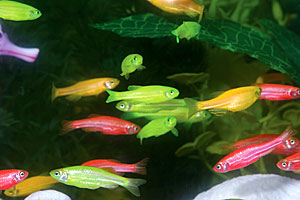
\includegraphics[width=\linewidth]{images/danio}
\caption{'Glofish':"Peces cebra"(\textit{Danio rerio}) que expresan proteínas fluorescentes GFP, YFP y RFP que actúan en asociación con el gen \textit{mylz2} \cite{gong2003development}}
%\label{fig:danio}
\end{figure}

  
%------------------------------------------------

\section{Implicancias Bioéticas de la Transfección}

Pese al enorme potencial de la transfección con sus innumerables aplicaciones, desde sus origenes ha existido un gran rechazo de múltiples grupos hacia esta tecnología. Esto se pudo observar por ciertas limitaciones legales a su investigación y uso en EEUU y Europa, particularmente en los años 80 \cite{Spink} .

%----------------------------------------------------------------------------------------
%	REFERENCE LIST
%----------------------------------------------------------------------------------------

\bibliographystyle{unsrt}
\bibliography{referencias}

%----------------------------------------------------------------------------------------

\end{document}
